\filesource.
Once you have downloaded the file, close any existing projects in your IDE, unpackage the file, and open the project in your IDE.\footnote{
    The starter code is prepared for use with PlatformIO.   % TODO - parameterize this?
    \textcolor{red}{If you are using the Arduino~IDE:}
    \begin{itemize}
        \item Go into the Arduino~IDE's Library Manager to see if you need to update the CowPi and/or CowPi\_stdio libraries.
        \item Move all source code out of the \textit{PollingLab/src/} directory and place it in the \textit{PollingLab/} directory.
        \item Rename \textit{PollingLab.cpp} as \textit{PollingLab.ino}.
    \end{itemize}
}
using these directions:\footnote{
    If you open the project directly in your IDE, your IDE may automatically detect that the project is a PlatformIO project and launch the PlatformIO plugin for you.
    We have seen that some students' IDEs do not automatically launch the PlatformIO plugin.
    If in doubt, launch the PlatformIO plugin and use it to open your project.
    \textit{Without the PlatformIO project active, you will not be able to build the project.}
}

\begin{description}
    \checkoffitem{Start your IDE.}
    \checkoffitem{Launch the PlatformIO plugin.}
    \checkoffitem{Depending on your particular IDE and plugin version, look for a button to ``Pick a Folder'', ``Open Project'', or something similar.}
    \checkoffitem{Click on that button and navigate to the PollingLab project.}
    \ifdefstring{\processor}{ATmega328P}{
        \checkoffitem{Open \textit{platformio.ini}.}
        \checkoffitem{If your Arduino~Nano uses the old bootloader, then use semicolons to comment-out the \texttt{env:nanoatmega328new} configuration settings and the \texttt{env:uno} configuration settings.}
        \checkoffitem{If your Arduino~Nano uses the new bootloader, then use semicolons to comment-out the \texttt{env:nanoatmega328old} configuration settings and the \texttt{env:uno} configuration settings.}
        \checkoffitem{Save \textit{platformio.ini}.}
    }{}
    \ifdefstring{\processor}{RP2040}{
        \checkoffitem{Build the project.}
            \begin{itemize}
                \item There are many parts of MBED~OS that generate compiler warnings.
                    By building the project now, before you've written any of your own code, you're assured that any compiler warnings that you see in the future will be warnings about \textit{your} code.
            \end{itemize}
    }{}
\end{description}


\subsection{Modes of Operation}

The switches' initial positions determine the mode of operation.

\subsubsection*{Test Keypresses and Time}

\begin{itemize}
    \item \textbf{left switch} in the \textit{right} position
    \item \textbf{right switch} in the \textit{right} position
\end{itemize}

\begin{description}
    \checkoffitem{Position both of your Cow~Pi's switches in the \textit{right} position.}
    \checkoffitem{Connect your computer to your Cow~Pi, open the Serial Monitor,\footnote{
            If you forgot to open the Serial Monitor, your Cow~Pi will pause for 5~seconds, waiting for you to open the Serial Monitor.
            If you do not do so before the connection attempt times out, your program will start while the Cow~Pi signals ``NO SERIAL'' in Morse Code.
        } and upload the program to your Cow~Pi.}
\end{description}
The display module will show: \\
\display{
    \colorbox{LightGreen}{KEYPRESS\phantom{xxxx}TIME} \vspace{-1mm}\\
    \colorbox{LightGreen}{\phantom{x}NO\phantom{xxxx}0.125260s}
} \\
and the right LED will be illuminated.

Whenever a key is pressed, the display will change \display{NO} to \display{YES}.
When that key is released, the display will change \display{YES} to \display{NO}.

Whenever a key is pressed or released, whenever a button is pressed or released, and whenever a switch is toggled,
the display will update to show the time elapsed since the microcontroller was powered up.

\subsubsection*{Test Inputs and Outputs}

\begin{itemize}
    \item \textbf{left switch} in the \textit{right} position
    \item \textbf{right switch} in the \textit{left} position
\end{itemize}

\begin{description}
    \checkoffitem{Position your Cow~Pi's \textbf{left switch} in the \textit{right} position, and the \textbf{right switch} in the \textit{left} position,
        and press the RESET button.}
\end{description}
The display module will show: \\
\display{
    \colorbox{LightGreen}{KEY\phantom{xxx}BTN\phantom{xxx}SW\phantom{x}} \vspace{-1mm}\\
    \colorbox{LightGreen}{\phantom{x}-\phantom{xxxx}U\phantom{x}U\phantom{xxx}R\phantom{x}L}
} \\

The display will show whether the buttons are pressed (``D'' for down) or not (``U'' for up)
and the positions of thw switches (``L'' for left, ``R'' for right).
The code that determines which key (if any) on the numeric keypad is pressed will work after you write a small amount of code in Section~\ref{subsec:populatekeypad}, which the TAs will guide you through.
If both pushbuttons are pressed, then the left LED will illuminate,
and if both switches are toggled to the right, then the right LED will illuminate.

\subsubsection{Simple Application}

\begin{itemize}
    \item \textbf{left switch} in the \textit{left} position
\end{itemize}

When the \textbf{left switch} is initially in the \textit{left} position, then the code that you will write in Section~\ref{sec:SimpleSystem} will run.


\subsection{Description of PollingLab Files}

% TODO: parameterize this

\subsubsection{io\_functions.h \& io\_functions.c}

Do not edit \textit{io\_functions.h}.

The \textit{io\_functions.c} file contains functions that you will edit in Sections~\ref{sec:LabTime} and Section~\ref{sec:MemMapIO}.
The functions that read the inputs and write to the outputs currently make use of CowPi library functions.
Your task will be to replace those library calls with code that uses the microcontroller's memory-mapped I/O registers.

% TODO: parameterize this

\subsubsection{number\_builder.h \& number\_builder.c}

Do not edit \textit{number\_builder.h}.

The \textit{number\_builder.c} file contains a function, \function{build_number()}, that the driver code will call when you are not running the I/O test,
and it contains helper functions that will address specific parts of building a number.
Right now these functions are only stubs.
In Section~\ref{sec:SimpleSystem}, you will write code in \function{build_number()} (and in helper functions of your devising) to implement a simple system's specification.

\subsubsection{PollingLab.cpp, starter-\lowercaseprocessor.cpp and starter.h}

Do not edit \textit{PollingLab.cpp}, \textit{starter-\lowercaseprocessor.cpp}, or \textit{starter.h}.


\subsection{Debouncing} \label{subsec:debouncing}

\begin{figure}[h]
    \centering
    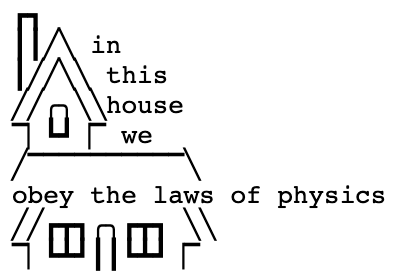
\includegraphics[height=3.5cm]{in-this-house}
\end{figure}

Mechanical buttons and switches demonstrate a phenomenon called \textit{switch bounce}.
This causes voltage to fluctuate for hundreds, often thousands, of microseconds when the contacts close or open.
When this fluctuation is in the indeterminate region between the logical low and high thresholds, it can cause the logic level to ``bounce'' back-and-forth between high and low until settling into the final, correct logic level.
This causes the digital circuitry or software to ``see'' multiple triggering events.

A traditional way to debounce is to introduce a simple low-pass filter using a resistor and a capacitor.
Other common hardware-based approaches use digital feedback circuits.
Hardware design can be simplified, and manufacturing cost can be reduced, by solving a hardware problem with software.
This, of course, transfers the design complexity to the software.

The CowPi library includes the \function{cowpi_debounce_byte()}, \function{cowpi_debounce_short()}, and \function{cowpi_debounce_long()}  functions that essentially implement a low-pass filter in software.
% TODO: parameterize io_functions.c
The functions in \textit{io\_functions.c} make use of \function{cowpi_debounce_byte()}.
When you modify these functions, as long as you preserve those \function{cowpi_debounce_byte()} calls, you do not need to worry further about debouncing.


\subsection{A Program in an Infinite Loop} \label{subsec:infiniteLoop}

As is common in embedded systems, after the program has been initialized, this assignment's program runs in an infinite loop:

% TODO: parameterize the functions being called
\begin{lstlisting}[numbers=none, basicstyle=\ttfamily\small]
static bool test_mode;

void setup() {
    initialize_board();
    test_mode = cowpi_left_switch_is_in_right_position();
    initialize_io(cowpi_right_switch_is_in_right_position());
    initialize_number_system();
}

void loop() {
    refresh_display();
    if (test_mode) {
        test_io();
    } else {
        build_number();
    }
}

int main() {
    setup();
    while(true) {
        loop();
    }
}
\end{lstlisting}


\subsection{Debugging} \label{subsec:debugging}

The starter code configures the Cow~Pi such that the \lstinline{stdout} file stream sends data to the Serial Monitor.
This allows you to print to the Serial Monitor using \function{printf()}.

\ifdefstring{\processor}{RP2040}{
% TODO: parameterize this (when we eventually port to the bare-metal Arduino toolchain, and to the Pico SDK)
    A consequence of this is that the development board will wait for the Serial Monitor to be ready, timing out after 5 seconds.
    If the connection attempt times out, then the \function{printf()} statements will have no effect, even if you later connect the Serial Monitor.

    If you wish to remove this configuration (thereby allowing the program to start immediately rather than wait for a Serial Monitor connection),
    then change the \lstinline{cowpi_setup(9600,} line in \textit{starter-rp2040.cpp} to \lstinline{cowpi_setup(0,}

    \textcolor{yellow}{
        If a Windows driver issue prevents you from printing to the Serial Monitor,
        then you can instead send short debug messages to the display module -- see Section~\ref{subsec:numberBuilderOutput} for information about outputting to the display module.
        The display module can display up to 8 rows of text, 16 characters per row;
        however, the assignment only makes use of rows~0 \& 1.
        This leaves rows~2--7 available for short (16 character) debug messages.
    }
}{}
